%!TEX TS-program = xelatex
\documentclass[a4paper, 12pt]{article}
\usepackage{barinovxesimple}
\geometry{top=25mm}
\geometry{bottom=35mm}
\geometry{left=35mm}
\geometry{right=20mm}
\setlist{labelindent=\parindent,leftmargin=*}
\begin{document}
\thispagestyle{empty}
\begin{center}
    \textit{Федеральное государственное автономное образовательное\\ учреждение высшего образования }

    \vspace{0.5ex}

        \textbf{«Московский физико-технический институт\\ (национальный исследовательский университет)»}
\end{center}

\vspace{10ex}

\begin{center}
    \vspace{13ex}

    \so{\textbf{Вопрос по выбору}}

    \vspace{1ex}

    по курсу общей физики

    на тему:

    \textbf{\textit{<<Униполярные
    двигатели>>}}

    \vspace{30ex}

    \begin{flushright}
        \noindent
        \textit{Работу выполнил:}\\  
        \textit{Баринов Леонид \\(группа Б02-827)}
    \end{flushright}
    \vfill
    Долгопрудный \\2020
\newpage
\setcounter{page}{1}
\fancyhead[R]{\nouppercase{\leftmark}}	
\end{center}

\section{Аннотация}

В работе будет определена контактная разность потенциалов
$(p-n)$-перехода в полупроводниковом диоде по результатам измерений
температурной зависимости его сопротивления.



\section{Теоретические сведения}
Приведем полупроводники $p$- и $n$- типа в соприкосновение, вызвав рекомбинацию электронов и дырок. При этом у границы перехода в $n$-области ионы донорной примеси образуют положительный пространственный заряд, а у границы перехода в $p$-области ионы акцепторной примеси --- отрицательный. Таким образом в области $(p-n)$-перехода возникает обедненный носителями тока слой и соответствующая \textbf{контактная разность потенциалов} --- барьер, препятствующий диффузии основных носителей. Равновесие возникает при совпадении уровней Ферми в $p$- и $n$-областях. Энергетическая схема перехода изображена на рисунке \ref{pic:energy_scheme}. 
	
	\begin{figure}[h]
		\centering	
		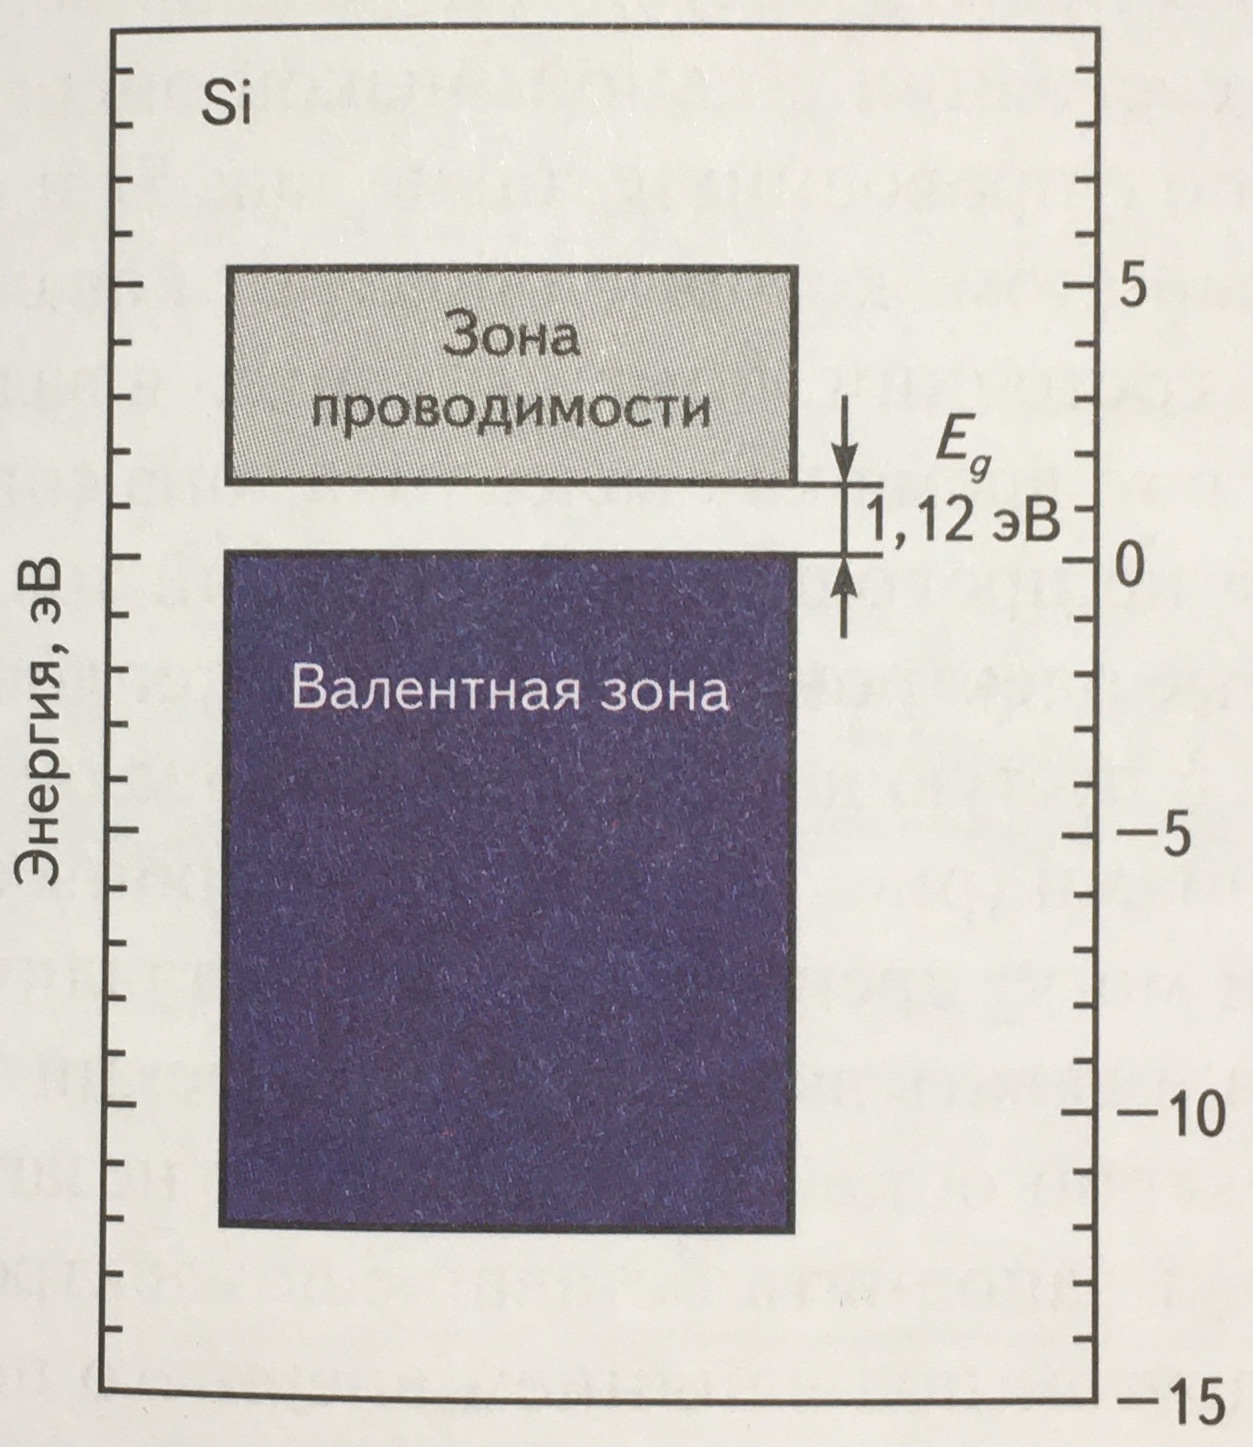
\includegraphics[width=0.6\textwidth]{1}
		\caption{Энергетическая схема $(p-n)$-перехода, находящегося в равновесии}
		\label{pic:energy_scheme}
	\end{figure}  
	
	На рисунке \ref{pic:energy_scheme} $E_c$ обозначена энергия,
        соответствующая дну зоны проводимости, $\mu$ --- уровень
        Ферми. В этих обозначениях при обычных температурах
        концентрация электронов $n_n$ в зоне проводимости и концентрация дырок $n_p$ в валентной зоне равны соответственно: 
	
	\[ n_n(n\text{-область}) = Q_n\exp\left(-\frac{E_c - \mu}{kT}\right) \]
	
	\[ n_p(p\text{-область}) = Q_p\exp\left(-\frac{\mu}{kT}\right) \]
	
	Из-за наличия контактной разности потенциалов $\Delta V$ между концентрациями основных и неосновных носителей тока в области устанавливается следующее соотношение:
	
	\[ \frac{n_n(n\text{-область})}{n_n(p\text{-область})} = \frac{n_p(p\text{-область})}{n_p(n\text{-область})} = \exp{\left(\frac{e\Delta V}{kT}\right)} \]
	
	Здесь индекс по-прежнему указывает на тип носителя, а в скобках стоит рассматриваемая область полупроводника.
	
	Проходящий через переход ток $I_0$ пропорционален концентрации неосновного заряда в области: 
	
	\[ I_0 \propto n_n(p\text{-область}) = n_n(n\text{-область}) \cdot \exp{\left(-\frac{e\Delta V}{kT}\right)} \]
	
	Приложим теперь к $(p-n)$-переходу напряжение $V_\text{ист}$ от внешнего источника, чтобы $p$-область заряжалась положительно относительно $n$-области (см. рисунок \ref{pic:external_voltage}.a). Потенциальный барьер снижается в $\exp{\left(\frac{eV_\text{ист}}{kT}\right)}$ раз, и ток, протекающий через переход слева направо, увеличивается в соответствующее количество раз. Ток справо налево остается неизменным и равен $I_0$. Тогда полный ток $I$ через барьер равен разности токов, текущих направо и налево: 
	
	\[ I = I_0\left(\exp\left(\frac{eV_\text{ист}}{kT}\right) - 1\right) \]
	
	Аналогичное равенство справедливо и для тока, переносимого дырками. 
	
	При приложении обратного напряжения (см. рисунок \ref{pic:external_voltage}.б)) полный ток также описывается формулой, данной выше.
	
	\begin{figure}[h]
		\centering	
		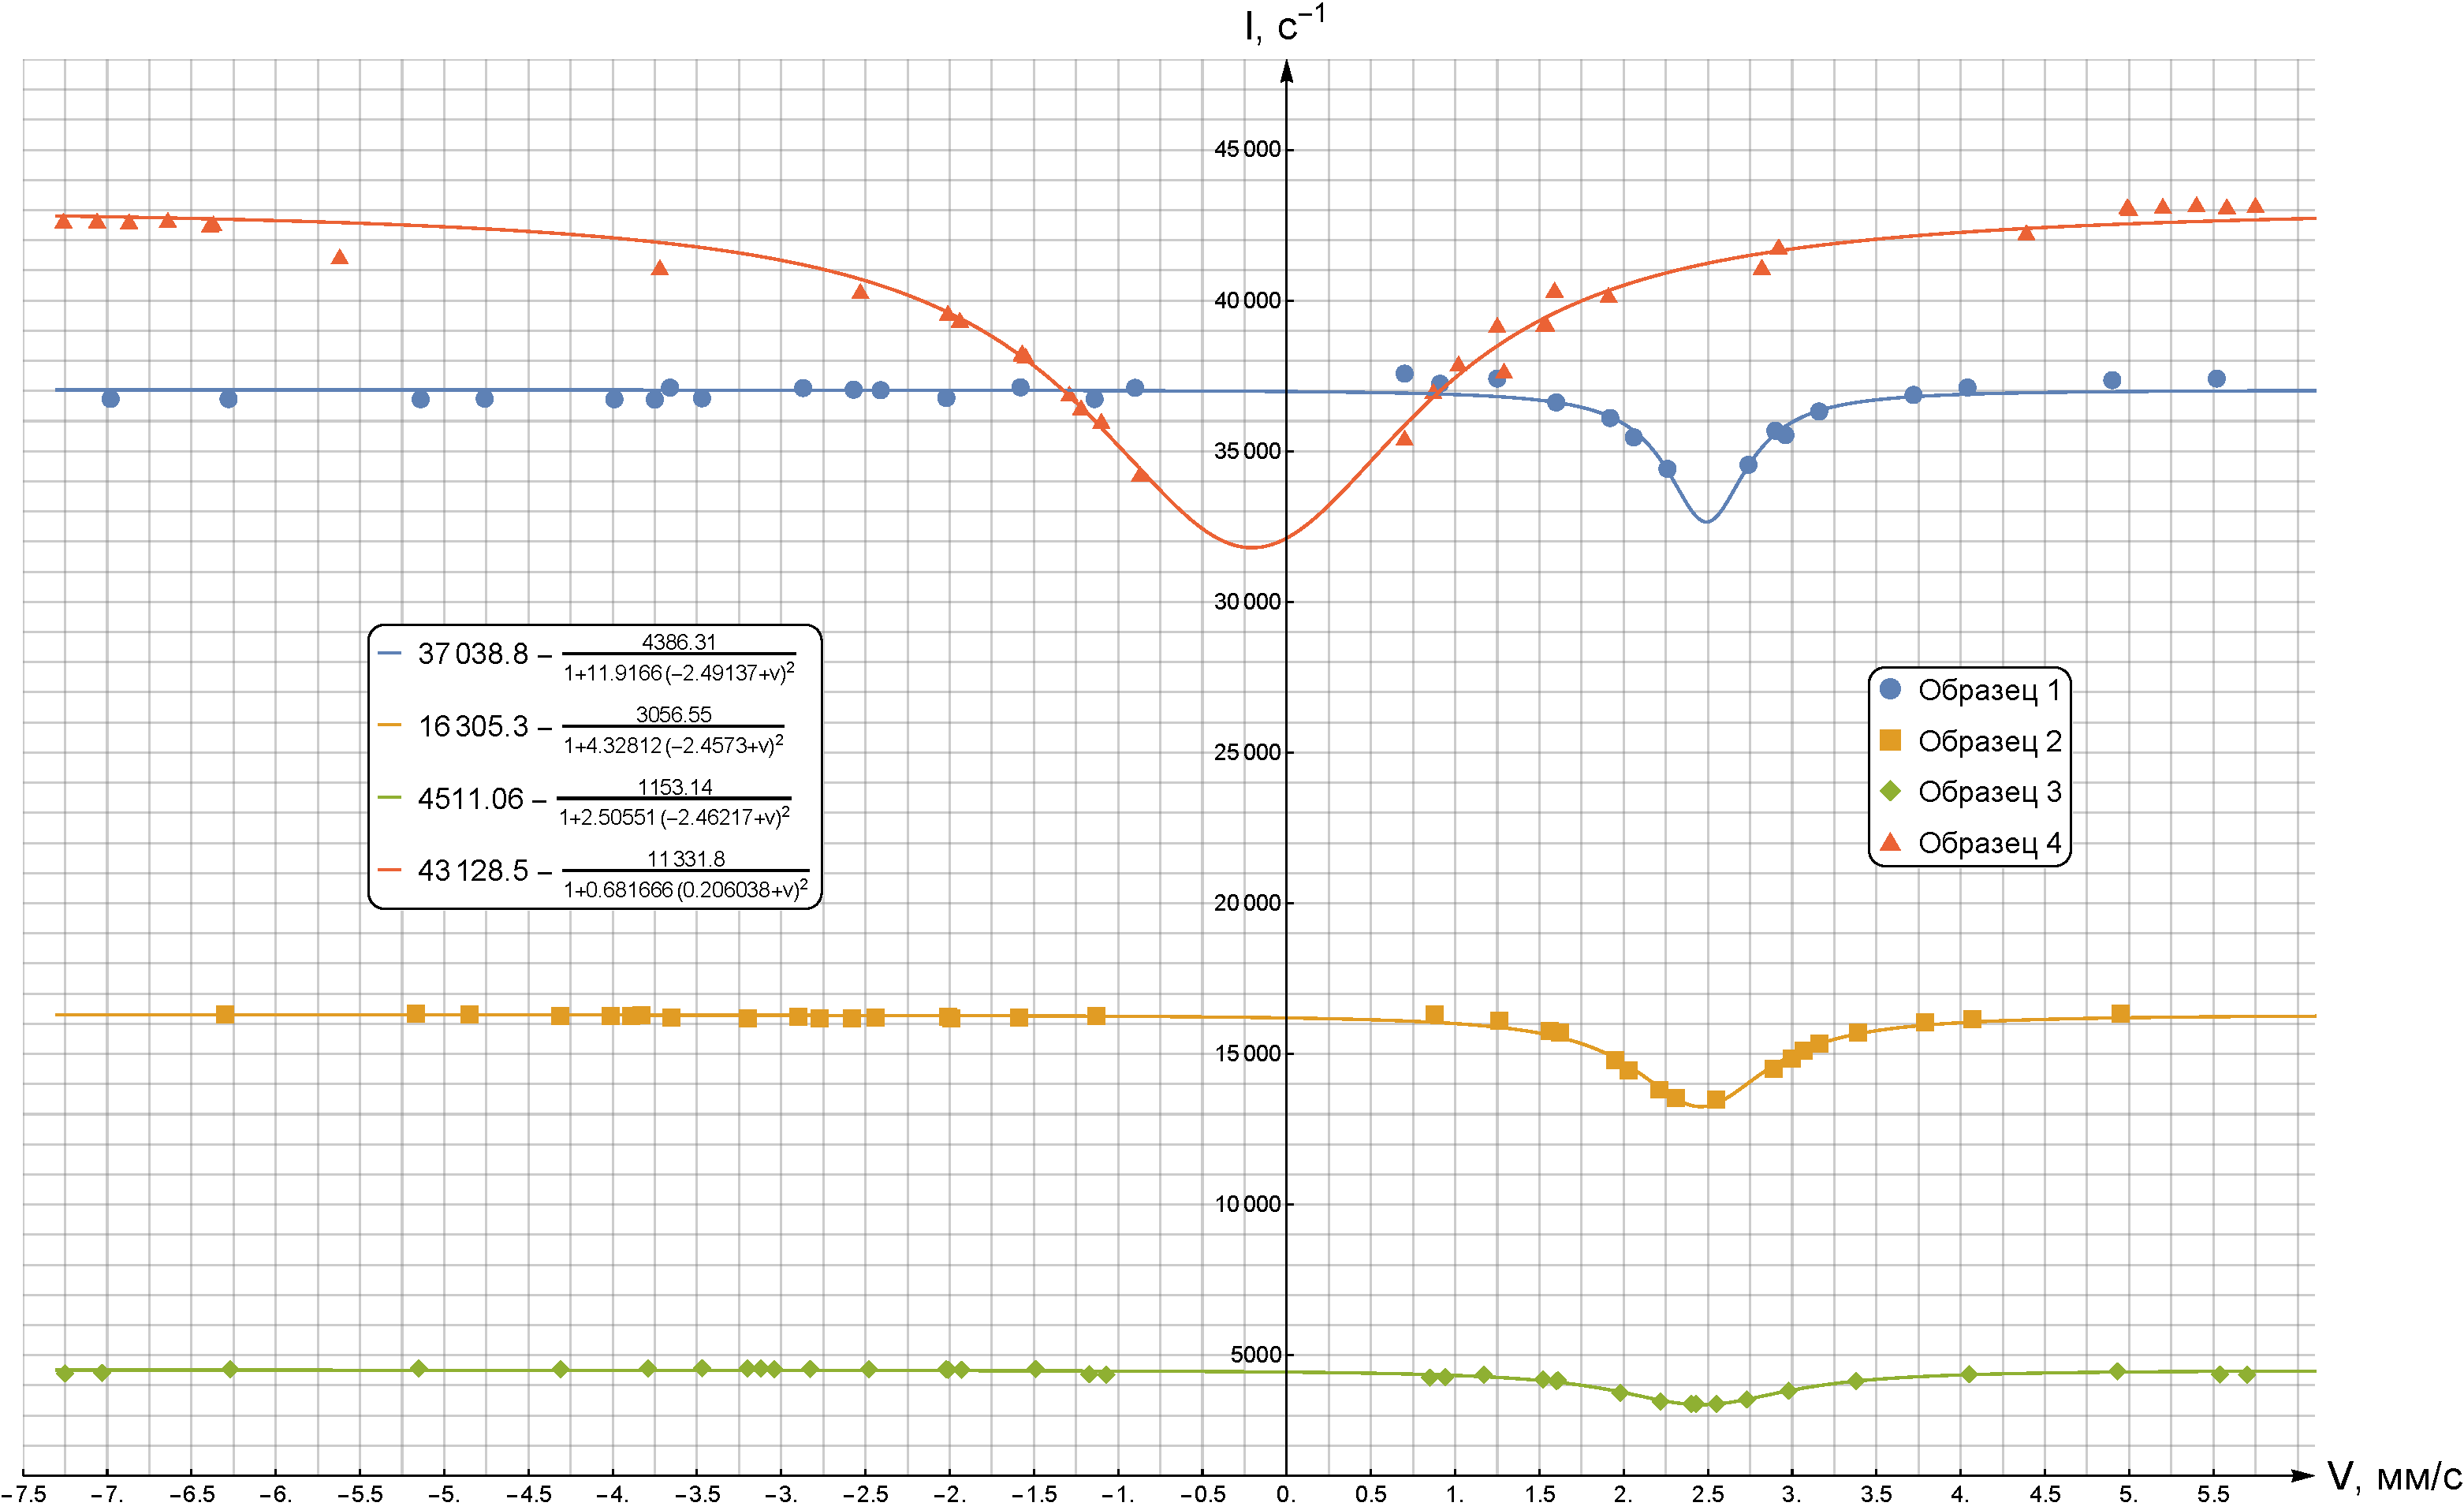
\includegraphics[width=0.5\textwidth]{2}
		\caption{Схема $(p-n)$-перехода под внешним напряжением с положительным (а) и отрицательным (б) смещениями области перехода}
		\label{pic:external_voltage}
	\end{figure} 
	
	Таким образом, при приложенном внешнем напряжении $V_\text{ист}$ суммарный ток электронов и дырок равен: 

        \begin{multline}
	 I = (I_{0, n} + I_{0, p})
         \left(\exp\left(\frac{eV_\text{ист}}{kT}\right) - 1\right) =
         \\= A(n_n(n\text{-область}) + n_p(p\text{-область})) \cdot
         \exp\left(-\frac{e\Delta
         V}{kT}\right)\left(\exp{\left(\frac{eV_\text{ист}}{kT}\right)}
     - 1\right) =\\ 
	 = C \exp\left(-\frac{e\Delta V}{kT}\right)\left(\exp{\left(\frac{eV_\text{ист}}{kT}\right)} - 1\right) 
    \end{multline}
	В последнем равенстве учтено, что концентрации электронов и дырок определяются концентрацией примесей и мало зависят от температуры. 
	
	При комнатных температурах справедливо приближение: $eV_\text{ист} \ll kT$. Тогда для полного тока через переход верно: 
	
	\[ I = C\exp{\left(-\frac{e\Delta V}{kT}\right)} \cdot \frac{eV_\text{ист}}{kT} \]
	
	Из полученного выражение для тока $I$ найдем сопротивление $R$ $(p-n)$-перехода: 
	
	\[ R = \frac{V_\text{ист}}{I} = \frac{1}{C} \cdot \frac{kT}{e} \exp{\left(\frac{e\Delta V}{kT}\right)} \propto \exp{\left(\frac{e\Delta V}{kT}\right)}\]
	
	При написании последнего равенства мы пренебрегли слабой зависимостью от температуры предэкспоненциального члена, которая
	мало заметна на фоне быстрой экспоненциальной зависимости.
	
	Логарифмируя и дифференцируя последнее выражение, получим искомую формулу для нахождения контактной разности потенциалов:
	
	\begin{equation}\label{dV}
	\Delta V = \frac{k}{e}\cdot \frac{\Delta(\ln R)}{\Delta(1/T)}
	\end{equation}







\section{Оборудование}


	Схема установки для измерения температурной зависимости контактной разности потенциалов $\Delta V(T)$ показана на рисунке \ref{pic:scheme}. Она состоит из мостиковой схемы и термостата. Источником питания схемы служит генератор прямоугольных импульсов, а сигнал с балансируемого моста подается на независимые каналы осциллографа.

		\begin{figure}[h]
		\centering
		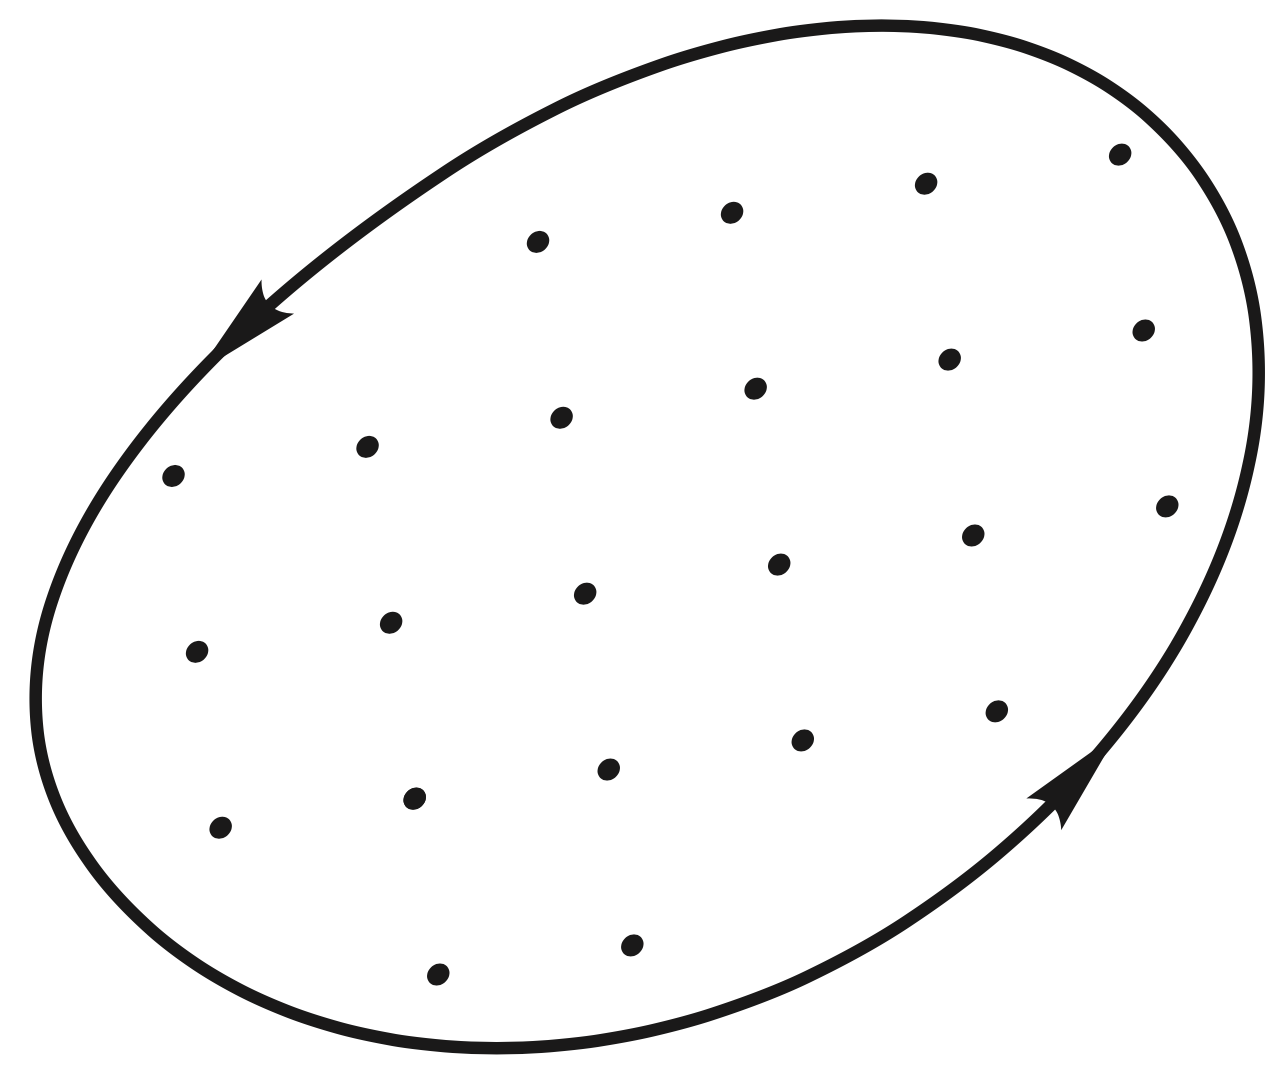
\includegraphics[width=0.6\textwidth]{3}
		\caption{Экспериментальная установка для определения контактной разности потенциалов $(p-n)$-перехода}
		\label{pic:scheme}
	\end{figure}


	На схеме на рисунке \ref{pic:scheme} указаны также номиналы используемых резисторов. Сопротивление диода $R$ выражается через сопротивление магазина $R_M$ и сопротивления $R_1 = 910$ Ом, $R_2 = 9.1$ кОм:

	\[ R = \frac{R_2}{R_1}R_M = 10\cdot R_M \]





\section{Результаты измерений и обработка результатов}

	Измерения проводятся в интервале температур от комнатной до
        $\approx 80^\circ$C. Температура образца измеряется медно-константановой термопарой, постоянная которой равна $\alpha = 41$ мкВ/K.


	Снимем зависимость сопротивления магазина $R_M$ при сбалансированном мосте от напряжения на термопаре $U$. По $R_M$ пересчитаем сопротивление диода $R = 10R_M$. Зная константу термопары $\alpha$,  получим температуру образца $T$ для соответствующего измерения напряжения:

        \[ T = T_0 + \frac{U}{\alpha} \]

	Измерения и последующие вычисления содержатся в таблице 1. 

\renewcommand{\arraystretch}{1.2}

\begin{table}[H]
\centering
\begin{tabular}{|>{$}c<{$}|>{$}c<{$}|>{$}c<{$}|>{$}c<{$}|>{$}c<{$}|>{$}c<{$}|>{$}c<{$}|>{$}c<{$}|>{$}c<{$}|}
\hline
\text{№} & U,\: мкВ & R,\: Ом & \Delta R,\: Ом & T,\: К      & 1/T,\:
К^{-1} & \Delta 1/T,\: К^{-1} & \ln R & \Delta \ln R \\ \hline
1  & 80     & 230   & 5            & 300,95 & 3,323 & 0,83  & 5,44 & 0,02   \\ \hline
2  & 180    & 180   & 5            & 303,39 & 3,296 & 0,37  & 5,19 & 0,03   \\ \hline
3  & 270    & 160   & 5            & 305,59 & 3,272 & 0,24  & 5,08 & 0,03   \\ \hline
4  & 390    & 123   & 4            & 308,51 & 3,241 & 0,17  & 4,81 & 0,03   \\ \hline
5  & 500    & 93    & 3            & 311,20 & 3,213 & 0,13  & 4,53 & 0,03   \\ \hline
6  & 620    & 80    & 3            & 314,12 & 3,183 & 0,10  & 4,38 & 0,04   \\ \hline
7  & 700    & 70    & 4            & 316,07 & 3,164 & 0,09  & 4,25 & 0,06   \\ \hline
8  & 800    & 63    & 3            & 318,51 & 3,140 & 0,08  & 4,14 & 0,05   \\ \hline
9  & 900    & 55    & 4            & 320,95 & 3,116 & 0,07  & 4,01 & 0,07   \\ \hline
10 & 1010   & 49    & 3            & 323,63 & 3,090 & 0,06  & 3,89 & 0,06   \\ \hline
11 & 1140   & 37    & 2            & 326,80 & 3,060 & 0,05  & 3,61 & 0,05   \\ \hline
12 & 1290   & 42    & 2            & 330,46 & 3,026 & 0,05  & 3,74 & 0,05   \\ \hline
13 & 1440   & 27    & 2            & 334,12 & 2,993 & 0,04  & 3,30 & 0,07   \\ \hline
14 & 1590   & 19    & 2            & 337,78 & 2,961 & 0,04  & 2,94 & 0,11   \\ \hline
15 & 1730   & 16    & 2            & 341,20 & 2,931 & 0,03  & 2,77 & 0,13   \\ \hline
\end{tabular}
\label{tab:1}
\caption{Результаты измерений}
\end{table}


\begin{figure}[H]
    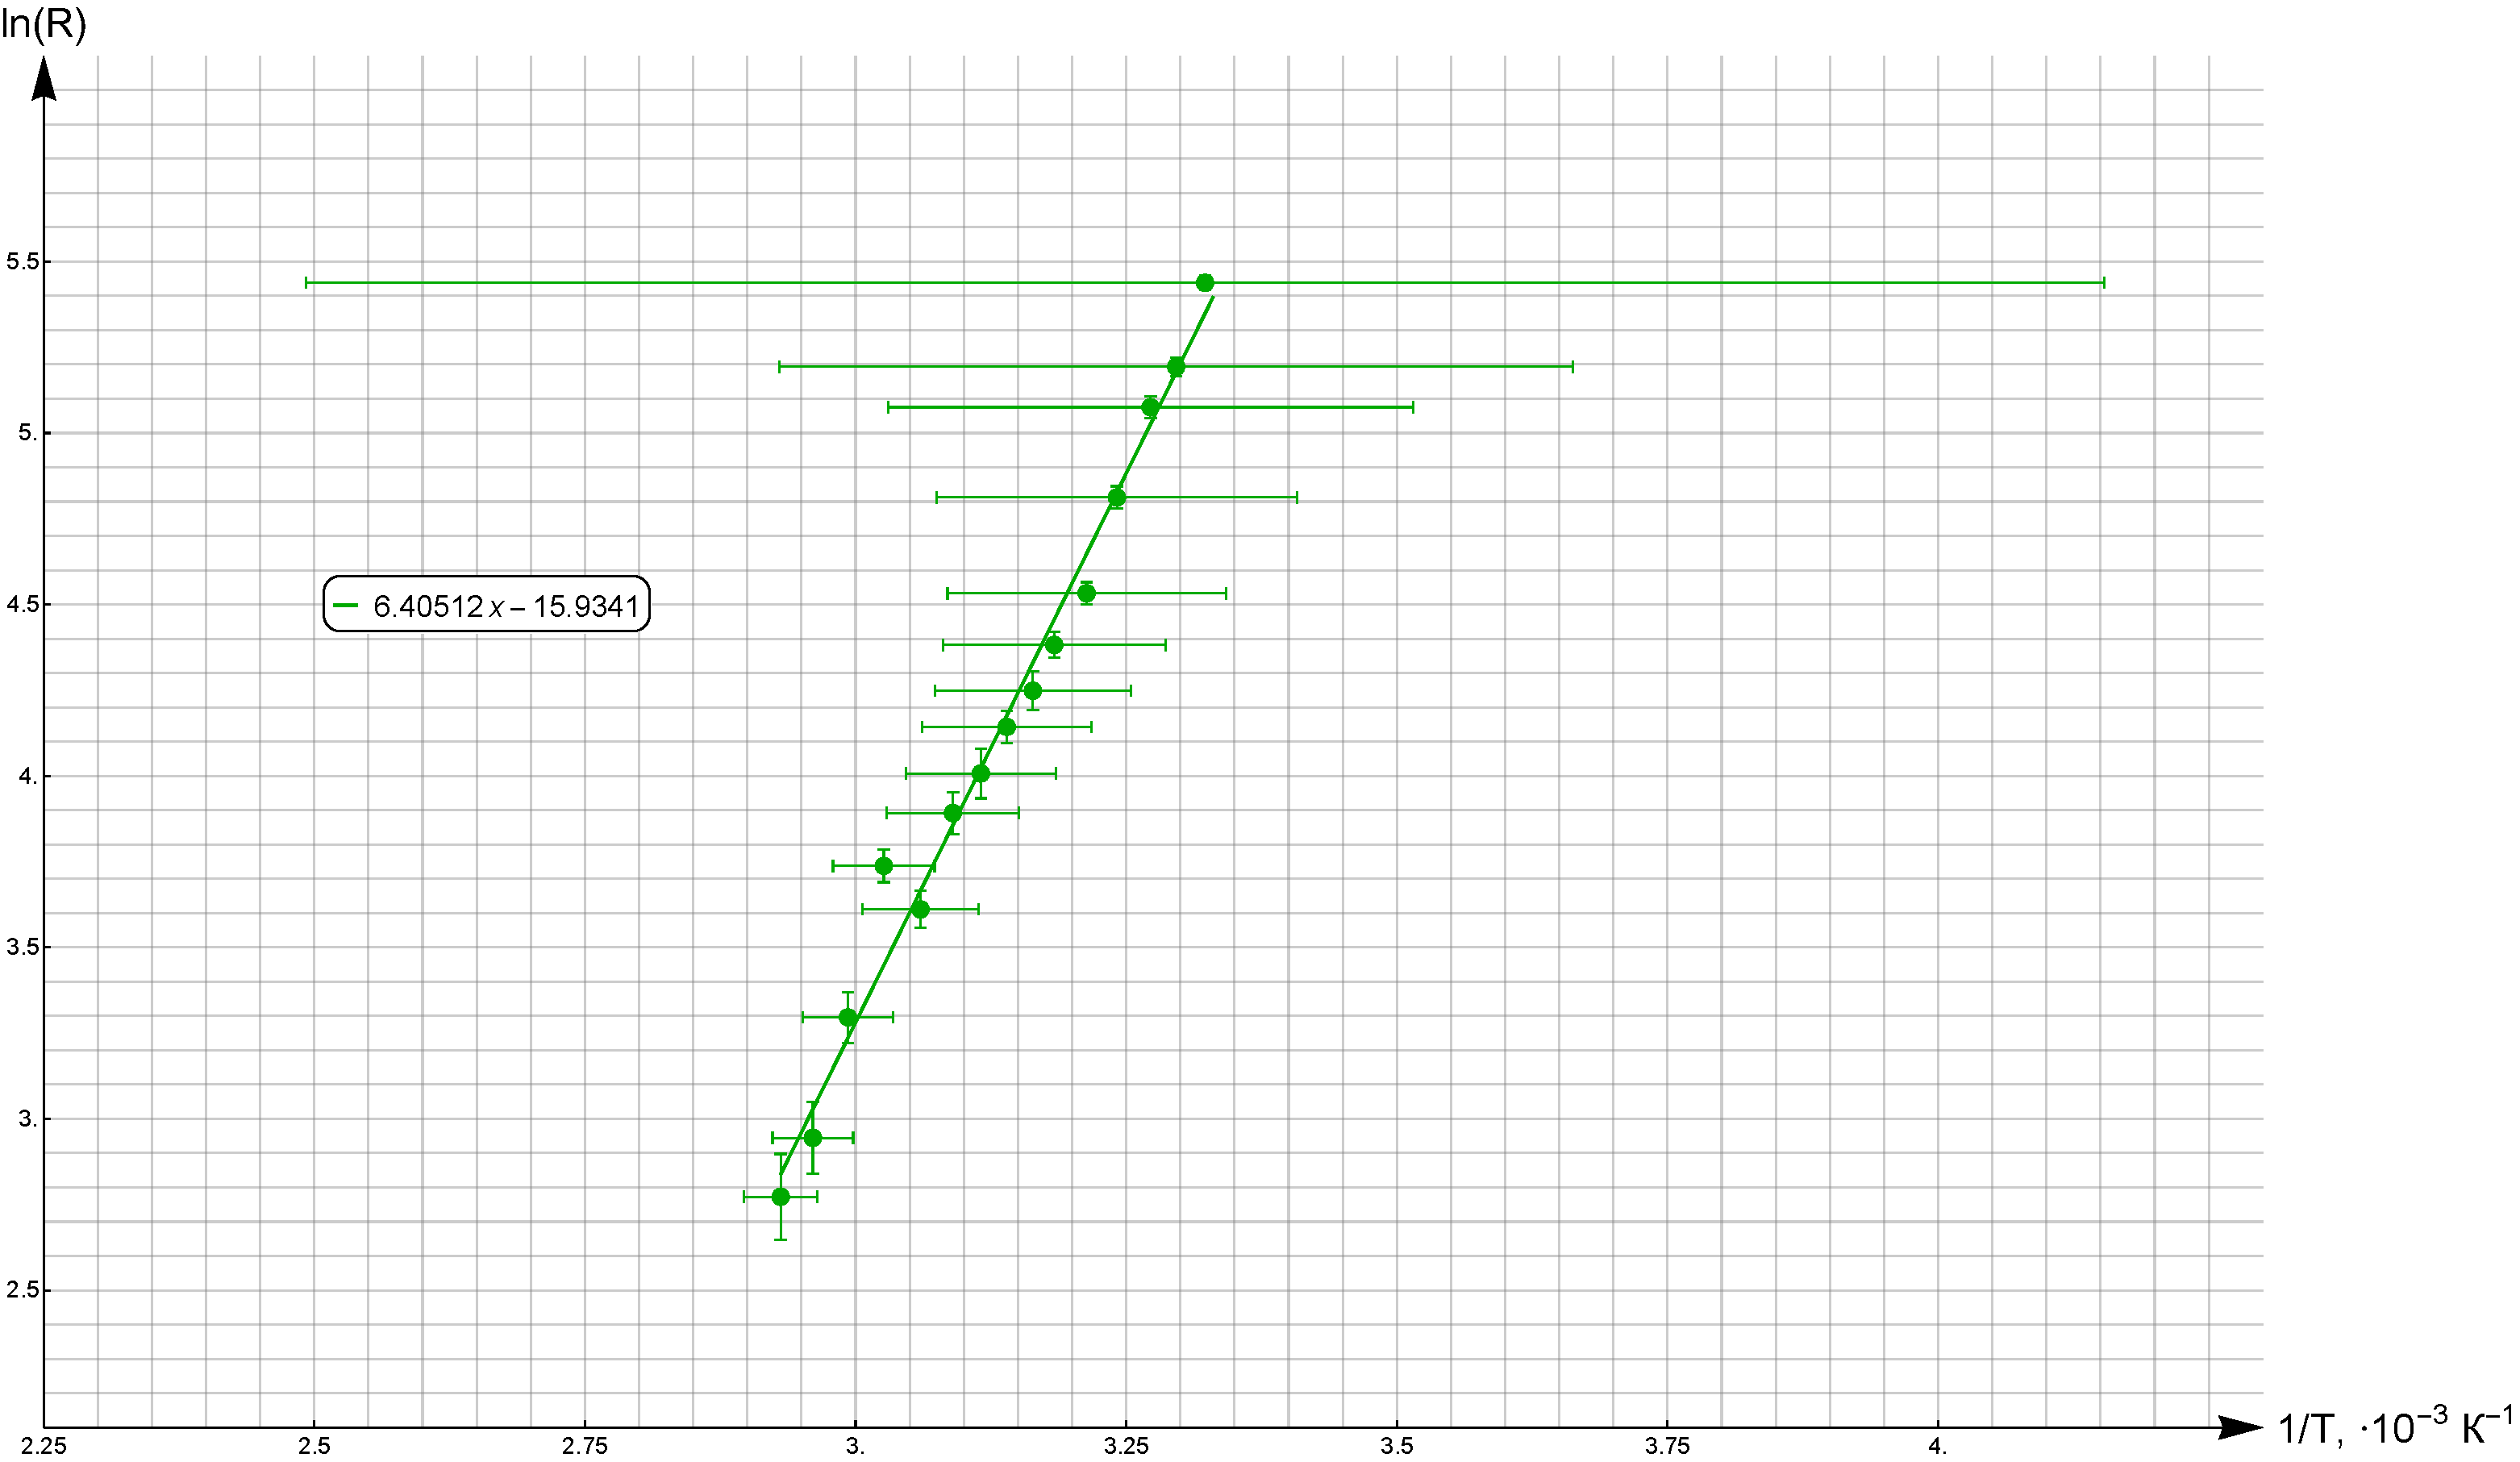
\includegraphics[width=1\linewidth]{line} 
    \caption{График зависимости $\ln R$ от $1/T$}
    \label{fig:1}
\end{figure}

Коэффицент наклона, полученные из аппроксимации:
\[
    k = (6,4 \pm 1,6)\: \cdot 10^3\: К^{-1}
\]

Находим искомую контактную разность
потенциалов $(p-n)$-перехода полупроводникового диода:
\[
    \Delta V = \frac{k_{B}}{e} \cdot k \approx (0,55 \pm 0,14)\: В 
\]










\section{Обсуждение результатов и выводы}
Контактная разность потенциалов $(p-n)$-перехода в полупроводниковом
диоде:
\[
    \Delta V = (0,55 \pm 0,14)\: В 
\]

Большая погрешность обуслевлена трудностью визуального определения
показаний осциллографа.















\end{document}
